% This is "aamas2012 .tex" August 2012 
% This file should be compiled with "aamas2012 .cls" 
% This example file demonstrates the use of the 'aamas2012 .cls'
% LaTeX2e document class file. It is for those submitting
% articles to AAMAS 2012  conference. This file is based on
% the sig-alternate.tex example file.
% The 'sig-alternate.cls' file of ACM will produce a similar-looking,
% albeit, 'tighter' paper resulting in, invariably, fewer pages.
% than the original style ACM style.
%
% ----------------------------------------------------------------------------------------------------------------
% This .tex file (and associated .cls ) produces:
%       1) The Permission Statement
%       2) The Conference (location) Info information
%       3) The Copyright Line with AAMAS data
%       4) NO page numbers
%
% as against the acm_proc_article-sp.cls file which
% DOES NOT produce 1) thru' 3) above.
%
% Using 'aamas2012 .cls' you don't have control
% from within the source .tex file, over both the CopyrightYear
% (defaulted to 200X) and the IFAAMAS Copyright Data
% (defaulted to X-XXXXX-XX-X/XX/XX).
% These information will be overwritten by fixed AAMAS 2012  information
% in the style files - it is NOT as you are used with ACM style files.
%
% ---------------------------------------------------------------------------------------------------------------
% This .tex source is an example which *does* use
% the .bib file (from which the .bbl file % is produced).
% REMEMBER HOWEVER: After having produced the .bbl file,
% and prior to final submission, you *NEED* to 'insert'
% your .bbl file into your source .tex file so as to provide
% ONE 'self-contained' source file.
%

\newtheorem{note}{Note}
\newtheorem{example}{Example}
\newtheorem{definition}{Definition}

% This is the document class for full camera ready papers and extended abstracts repsectively 

\documentclass{aamas2012}

\usepackage{graphicx}
\usepackage{color}
\usepackage{algorithm,algorithmic}

\graphicspath{{pictures/}}

% if you are using PDF LaTex and you cannot find a way for producing
% letter, the following explicit settings may help
 
\pdfpagewidth=8.5truein
\pdfpageheight=11truein

\begin{document}

% In the original styles from ACM, you would have needed to
% add meta-info here. This is not necessary for AAMAS 2012  as
% the complete copyright information is generated by the cls-files.


\title{Representing Agent Reasoning With Meta-Knowledge on ASP Modules Combination}

% AUTHORS


% For initial submission, do not give author names, but the
% tracking number, instead, as the review process is blind.

% You need the command \numberofauthors to handle the 'placement
% and alignment' of the authors beneath the title.
%
% For aesthetic reasons, we recommend 'three authors at a time'
% i.e. three 'name/affiliation blocks' be placed beneath the title.
%
% NOTE: You are NOT restricted in how many 'rows' of
% "name/affiliations" may appear. We just ask that you restrict
% the number of 'columns' to three.
%
% Because of the available 'opening page real-estate'
% we ask you to refrain from putting more than six authors
% (two rows with three columns) beneath the article title.
% More than six makes the first-page appear very cluttered indeed.
%
% Use the \alignauthor commands to handle the names
% and affiliations for an 'aesthetic maximum' of six authors.
% Add names, affiliations, addresses for
% the seventh etc. author(s) as the argument for the
% \additionalauthors command.
% These 'additional authors' will be output/set for you
% without further effort on your part as the last section in
% the body of your article BEFORE References or any Appendices.

%\numberofauthors{8} %  in this sample file, there are a *total*
% of EIGHT authors. SIX appear on the 'first-page' (for formatting
% reasons) and the remaining two appear in the \additionalauthors section.
%

\numberofauthors{3}

\author{
% You can go ahead and credit any number of authors here,
% e.g. one 'row of three' or two rows (consisting of one row of three
% and a second row of one, two or three).
%
% The command \alignauthor (no curly braces needed) should
% precede each author name, affiliation/snail-mail address and
% e-mail address. Additionally, tag each line of
% affiliation/address with \affaddr, and tag the
% e-mail address with \email.
% 1st. author
\alignauthor
Tony Ribeiro\\
       \affaddr{National Institute of Informatics}\\
       \affaddr{Tokyo, Japan}\\
       \email{ribeiro@nii.ac.jp}
% 2nd. author
\alignauthor
Katsumi Inoue\\
       \affaddr{National Institute of Informatics}\\
       \affaddr{Tokyo, Japan}\\
       \email{ki@nii.ac.jp}
% 3rd. author
\alignauthor
Gauvain Bourgne\\
       \affaddr{????}\\
       \affaddr{Paris, France}\\
       \email{bourgne@nii.ac.jp}
}

%\and  % use '\and' if you need 'another row' of author names

% 4th. author
%\alignauthor Lawrence P. Leipuner\\
%       \affaddr{Brookhaven Laboratories}\\
%       \affaddr{Brookhaven National Lab}\\
%       \affaddr{P.O. Box 5000}\\
%       \email{lleipuner@researchlabs.org}

% 5th. author
%\alignauthor Sean Fogarty\\
%       \affaddr{NASA Ames Research Center}\\
%       \affaddr{Moffett Field}\\
%       \affaddr{California 94035}\\
%       \email{fogartys@amesres.org}

% 6th. author
%\alignauthor Charles Palmer\\
%       \affaddr{Palmer Research Laboratories}\\
%      \affaddr{8600 Datapoint Drive}\\
%       \affaddr{San Antonio, Texas 78229}\\
%       \email{cpalmer@prl.com}

%\and

%% 7th. author
%\alignauthor Lawrence P. Leipuner\\
%       \affaddr{Brookhaven Laboratories}\\
%       \affaddr{Brookhaven National Lab}\\
%       \affaddr{P.O. Box 5000}\\
%       \email{lleipuner@researchlabs.org}

%% 8th. author
%\alignauthor Sean Fogarty\\
%       \affaddr{NASA Ames Research Center}\\
%       \affaddr{Moffett Field}\\
%       \affaddr{California 94035}\\
%       \email{fogartys@amesres.org}

%% 9th. author
%\alignauthor Charles Palmer\\
%       \affaddr{Palmer Research Laboratories}\\
%       \affaddr{8600 Datapoint Drive}\\
%       \affaddr{San Antonio, Texas 78229}\\
%       \email{cpalmer@prl.com}

%}

%% There's nothing stopping you putting the seventh, eighth, etc.
%% author on the opening page (as the 'third row') but we ask,
%% for aesthetic reasons that you place these 'additional authors'
%% in the \additional authors block, viz.
%\additionalauthors{Additional authors: John Smith (The Th{\o}rv{\"a}ld Group,
%email: {\texttt{jsmith@affiliation.org}}) and Julius P.~Kumquat
%(The Kumquat Consortium, email: {\texttt{jpkumquat@consortium.net}}).}
%\date{30 July 1999}
%% Just remember to make sure that the TOTAL number of authors
%% is the number that will appear on the first page PLUS the
%% number that will appear in the \additionalauthors section.

\maketitle

\begin{abstract}
	In this work, our interest is about multi-agent systems in dynamic environment.
	Here, we focus on representation of agent knowledge and reasoning.
	For reasoning in such environment, an agent needs to be able to manage his knowledge in a non-monotonic way.
	To reach his goals in a changing context, an agent needs to adapt his believes and behaviour regarding the current state of the world.
	Our objective is to define a method which makes easier to design agent knowledge and reasoning in such environment.
	For this purpose, we use the expressibility of answer set programming to propose a method based on ASP modules combinations.
	By using meta-knowledge on these combinations we represent dynamic behaviours and meta-reasoning.
	We also propose a framework to implement and use this method in multi-agent systems.
\end{abstract}

% Note that the category section should be completed after reference to the ACM Computing Classification Scheme available at
% http://www.acm.org/about/class/1998/.

\category{H.4}{Information Systems Applications}{Miscellaneous}

%A category including the fourth, optional field follows...
%\category{D.2.8}{Software Engineering}{Metrics}[complexity measures, performance measures]

%General terms should be selected from the following 16 terms: Algorithms, Management, Measurement, Documentation, Performance, Design, Economics, Reliability, Experimentation, Security, Human Factors, Standardization, Languages, Theory, Legal Aspects, Verification.

\terms{Design}

%Keywords are your own choice of terms you would like the paper to be indexed by.

\keywords{Multi-Agents System, Answer Set Programming, Meta-knowledge, ASP modules}

\section{Introduction}

	In this work we consider an agent as an entity which is able to reason and communicate with his fellows.
	We divide the knowledge of an agent in two part:\newline
		\begin{itemize}
			\item $K$ a set of not revisable knowledge composed of :
			\begin{itemize}
				\item $T$ the common theory
				\item $O$ the current observations
			\end{itemize}
			\item $B$ a set of revisable knowledge
		\end{itemize}
	
	$T$ is the common knowledge of all agent of a multi-agent system, it is considered as certain and not revisable.
	A common theory can also be limited to a group of agent which does not contain all the system.
	Observations are informations retrieved from the environment, it represents the current state of the world.
	If we consider that sensors are perfect then a current observation is not revisable.
	At time step 0, the knowledge of an agent is his common theory.
	This knowledge is extended by adding observations and its consequences at each new time step.

	$B$ is agent's beliefs, it represent informations supposed as true by the agent and which are revisable.
	In a dynamic environment, if current observations are certain, it is not the case of past ones.
	If an agent assume that past observations are correct until new ones prove the contrary his memory is a part of his beliefs.
	For example if an agent $a$ see an agent $b$ at position $p$ at time $T$.
	At $T+1$, $a$ does not see any more the position $p$ but he also does not see agent $b$.
	Then $a$ can assume that $b$ is always at position $p$ at $T+1$ and when $a$ will see again the position $p$ or $b$ he will revise his memory if needed.

	In recent years, many works focus on specific aspect of multi-agents systems such as communications, reasoning, learning or planning.
	Regarding communications, in \cite{DBLP:conf/ecai/BourgneIM10, DBLP:conf/lads/BourgneIM10} authors are interesting 
	by propagation of information in a group of agent.
	There is also interesting works like \cite{DBLP:conf/ijcai/SakamaSP11}, where agents can lie to achieve their goals.
	In this work, agents are in competition and tried to persuade others agents to reach their objectives.
	Others work focus on group planning, in \cite{DBLP:conf/clima/NieuwenborghVHV06} they consider a hierarchy between agent of a MAS.
	This hierarchy allows more flexibility of planning by prefer satisfaction of hight grade agent.
	Its also simplify communications between agents: an agent does not have to justify his choice to his subordinate.
	
	Our interest is about representing agent reasoning in dynamic environment.
	In Multi-agents systems, reasoning in dynamic environment implies to deal with some interesting problems.
	In such environment, an agent has to adapt to the evolution of the world to achieve his goals.
	His knowledge have to be updated regarding world changes by adding new observations or revising old ones.
	The behaviour of an agent needs to be suitable to the current situation and able to evolve with it.
	Designing such kind of reasoning is an interesting challenge which is the purpose of this work.
	
	To make our work more understandable we will follow an intuitive example along our propositions: a survival game which represent a MAS in a dynamic environment.
	In this game there are three groups of agents: wolfs, rabbits and flowers.
	Each kind of agent have specific goals and behaviours.
	To be simple, wolfs eat rabbits and rabbits eat flowers.
	
	Wolfs have only one goal: feed themselves.
	To reach this goal they have to catch and eat rabbits.
	A wolf can be in two situations: a prey is in sight or not.
	If there is no rabbit in the sight range of a wolf, the predator have to explore his environment to find one.
	When a prey is spotted, a wolf will try to perform a sneaky approach if he is not spotted himself, otherwise the predator will rush on his target.
	To resume, a wolf have three behaviours: exploration, approach and attack.
	
	Rabbits have two goals : feed and not be eat.
	On a first hand, a rabbit have to eat flowers and on an other hand it have to escape from wolf.
	Like a wolf, if no prey is in sight a rabbit need to explore its environment.
	But by doing this, a rabbit can find preys or predators.
	The exploration behaviour of a rabbit is more complex than the one of a wolf.
	For example: when a rabbit move it can choose the position with the best sight range for easily spotted its predators.
	When a wolf is spotted, survive is more important than feed then a rabbit have to hide or run away.
	To resume, a rabbit have four behaviours: exploration, feed, hide and run away.
	In this paper our examples will focus on rabbit agent for knowledge representation and reasoning.
	
	Flowers are passive agents: the environment have no effect on their behaviour.
	The only goal of a flower is to reproduce.
	A flower produce regularly a new one after a certain amount of time.
	Knowledge of a flower does not change regarding time.
	A flower is an independent agent, it does not care about others agents.

	\begin{figure}
		\centering
		
\includegraphics[keepaspectratio=true,scale=3.0]{food_chain.png}
		\caption
		{
			\label{food_chain}
			A MAS in a dynamic environment where an agent is a wolf, a rabbit or a flower:
			Wolfs eat rabbits and rabbits eat flowers.
		}
	\end{figure}
	
	Answer set programming which is a specification and an implementation language is very suitable to represent agent knowledge and reasoning.
	The methods introduce by this work is based on ASP modules and their combinations.
	ASP modules allows to represent agent behaviours in an intuitive and elegant way.
	We divide agent knowledge into different modules and use different modules combinations for reasoning.
	It allows agent to perform meta-reasoning: they use knowledge on modules combinations to adapt their reasoning and so on their behaviour to the situation.

\section{Answer set programming}

	\begin{definition}[Rule]
		Let $H$, $a_{i}$ and $b_{i}$ literals and the rule
	
					$$H \leftarrow a_{1}, \ldots , a_{n}, \neg b_{1} \ldots, \neg b_{m}.$$
		If all $a_{i}$ are true and all $b_{i}$ are not true then $H$ is true.
		$H$ is the head of the rule and the conjunction of $a_{i}$, $\neg b_{i}$ is the body.
	\end{definition}

	Answer set programming (ASP) is a form of declarative programming based on the stable model semantics of logic programming.
	An ASP program describes a problem, not how to solve it.
	Such program is composed of facts, rules and constraints. 
	Rule with an empty body: $H.$ are facts.
	Rules without head: $\leftarrow a_{1}, \ldots , a_{n}, \neg b_{1} \ldots, \neg b_{m}.$ are constraints.
	When conditions of constraints are evaluated as true its imply $\bot$.
	In this paradigm the search of solution is resume to compute answer sets of ASP program.
	An answer set is a set of facts which is consistent with all constraints of the program, its facts are deduce from facts and rules of the program.
	To compute it we run a solver on such program.
	
	\begin{example}
		\label{ASP_example}
		An ASP program composed of one fact, three rules and one constraint :\newline
		\newline
		rain.\newline
		stay $\leftarrow$ not go\_out.\newline
		go\_out $\leftarrow$ not stay.\newline
		wet $\leftarrow$ rain, go\_out, not umbrella.\newline
		$\leftarrow$ wet.
	\end{example}
	
	In example \ref{ASP_example} \{\emph{rain}, \emph{stay}\} is an answer set of this ASP program but \{\emph{rain}, \emph{go\_out}, \emph{wet}\} is not, 
	because it is not consistent with the constraint.
	
	Many research work concern ASP or use it to represent knowledge such as \cite{DBLP:conf/atal/BaralGSP10} or \cite{DBLP:conf/clima/NieuwenborghVHV06}.
	In the first one, the authors use it to represent the knowledge of an agent about the knowledge of others agents.
	In the second one, they focus on the flexibility of reasoning by introducing soft constraints: constraints which can be violate in some case.
	Others works like \cite{DBLP:conf/datalog/Costantini10} design ASP methods to improve some specific property of agent reasoning.
	In this work the author focus on reactivity by using ASP modules where constraints are used as actions trigger.
	In \cite{DBLP:conf/lpnmr/Costantini09}, the author discuss about integration of ASP modules into agent reasoning.
	There is also works like \cite{DBLP:conf/aaaiss/BaralAD06} or \cite{DBLP:conf/birthday/FaberW11} where they discuss about possible extensions of ASP paradigm.

\section{ASP modules}

	An ASP module is an ASP program which have a specific form and a specific use.
	The first advantage of these modules is their simplicity: a module is a little program which represent a specific knowledge.
	We can have a module which contain observations about surroundings,
	an other one to define what is a prey and a module dedicated to compute path.
	By combining this three modules an agent can compute all paths to surroundings preys.
	To design agent knowledge we respect a module typology to represent background knowledge, observations and meta-knowledge.

\subsection{Typology}

	\begin{definition}[Background module]
		A background module is a set of rules which represent knowledge about a specific domain.
		The set of all background modules of an agent represent his background knowledge.
		The purpose of these modules is to organise knowledge representation and produce
		new knowledge by combining it with others modules.
	\end{definition}
	
	Example \ref{rules_example} show two background modules, the first one represent knowledge about agent possibility of movement and 
	the second one represent knowledge about movement as an action.
	To simplify the first module of this example, \textit{distance/3} is supposed given by an other module and 
	his third argument is the distance between an agent A and a position P.
	Predicate \textit{action/2} specify the number of action that an agent can perform in one time step.
	The first module can be use by a rabbit to compute his movement possibility and the ones of his predator.
	The second module define the movement action, it specify that only one move can be perform and it should not be in the movement range of a wolf.
	By combining this two modules with observations about wolf a rabbit will produce all possible movement which are not in the direct movement range of any wolf.
	
	\begin{example}
		\label{rules_example}
		A background module of a rabbit about movement where A is an agent, P a position and S a number of step:\newline
		\newline
		reachable(A,P,S) $\leftarrow$ distance(A,P,S).\newline
		reachable(A,P) $\leftarrow$ reachable(A,P,S), action(A,S).
		\newline
		A background module about actions:\newline
		\newline
		action(me,3).\newline
		action(wolf,4).\newline
		0\{move(me,P)\}1 $\leftarrow$ reachable(me,P).\newline
		$\leftarrow$ move(A,P1), move(A,P2), P1 != P2.\newline
		$\leftarrow$ move(me,P), reachable(wolf,P).
	\end{example}

	\begin{definition}[Observations module]
		An observations module is a set of facts which represent related observations.
		The content of such module is dynamic: it change regarding time.
		The set of all observations modules of an agent represent his memory: current and past observations.
		The purpose of these modules is to organise observations to facilitate their use and update.
	\end{definition}
	
	\begin{example}
		An observations module of a rabbit about wolfs positions :\newline
		\newline
		position(wolf,0,3).\newline
		position(wolf,2,5).\newline
		position(wolf,2,6).\newline
		\newline
		An observations module of a rabbit about himself : \newline
		\newline
		me("Bugs Bunny").\newline
		position("Bugs Bunny",0,0).\newline
		type("Bugs Bunny",rabbit).\newline
	\end{example}

	With this two kind of modules we can represent the background theory and observations of an agent.
	The idea now is that we can combine our modules to produce different kind of knowledge.
	The figure \ref{module_combination} represent the knowledge of a rabbit by a set of observations modules and background modules.
	In this example, by combining modules \emph{Myself}, \emph{Field} and \emph{Move} a rabbit will produce all his possibility of movement.
	The combination \{\emph{Rabbit}, \emph{Field}, \emph{Move}\} will produce all possible movements that others rabbits can perform. 
	By combining \{\emph{Myself}, \emph{Field}, \emph{Flower}, \emph{Move}, \emph{Eat}, \emph{Action}\} 
	a rabbit will produce all possible actions he can perform now and their influence on the number of step needed to eat each flower.
	
	We can see here a first advantage of knowledge modularity: a module can be used for multiple purpose.
	If we take the example of modules \emph{Move} and \emph{Eat}, an agent can use it to reason about its possibilities and the ones of other agent.
	
	\begin{figure}
		\centering
		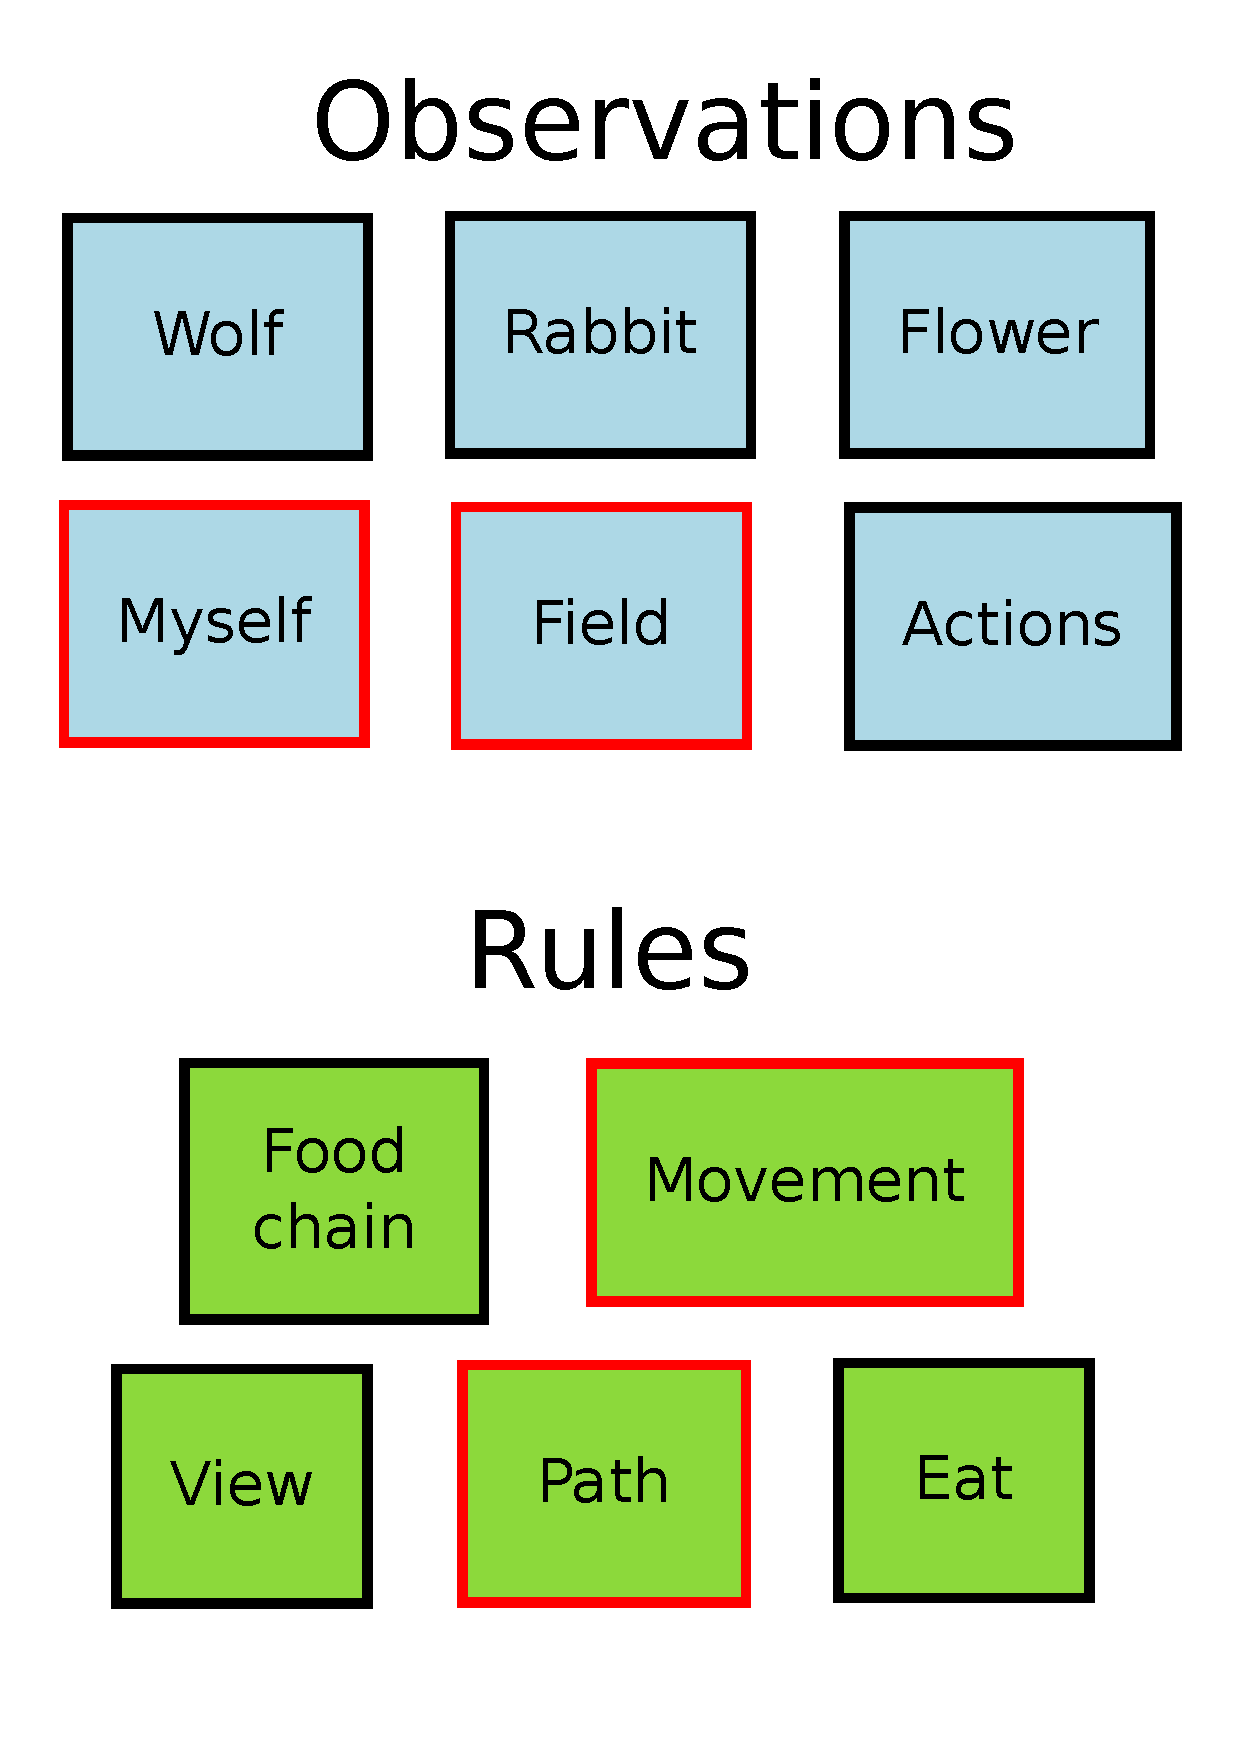
\includegraphics[keepaspectratio=true, scale=0.4]{module_combination.pdf}
		\caption
		{
			\label{module_combination}
			Knowledge base of a rabbit divided into observations modules (dot ones) and background modules (plain ones).
		}
	\end{figure}

	We have presented different way to use agent knowledge via module combination.
	But these combinations are also a kind of knowledge and it can be known by the agent.
	For the agent it is meta-knowledge on his knowledge, more precisely in this case it is knowledge about the use of his knowledge.
	This meta-knowledge is a part of the background theory of an agent and could be represented by background modules.
	But to clarify the design of agent knowledge we dedicated a new kind of modules to represent it.

	\begin{definition}[Meta-knowledge module]
		A meta-knowledge module is a set of rules which define the conditions to use ASP modules combinations.	
		The purpose of these modules is to represent dynamic behaviours by performing decision on how to reason and use knowledge.
	\end{definition}
	
	A module combination can represent agent behaviour and by using meta-knowledge modules we can represent it in a elegant way.
	Most simple behaviour can be represented by a simple list of modules to combine, like in examples \ref{run_away_example}, 
	\ref{feed_example} and figures \ref{run_away_figure}, \ref{feed_figure}.
	The module combination \{\emph{Myself}, \emph{Wolf}, \emph{Field}, \emph{Move}, \emph{Eat}, \emph{Action}\} 
	and \{\emph{Myself}, \emph{Rabbit}, \emph{Flower}, \emph{Field},  \emph{Move}, \emph{Eat}, \emph{Action}\} 
	can respectively represent the \textit{run away} and the \textit{feed} behaviour of a rabbit.
	This two combinations of modules can be represented by meta-knowledge modules, in this case theses modules have knowledge on background and observations modules.
	
	\begin{example}
		\label{run_away_example}
		A meta-knowledge module which describe the approach behaviour of wolf:\newline
		\newline
		\textbf{use\_module}("Myself").\newline
		\textbf{use\_module}("Wolf").\newline
		\textbf{use\_module}("Field").\newline
		\textbf{use\_module}("Move").\newline
		\textbf{use\_module}("Eat").\newline
		\textbf{use\_module}("Action").
	\end{example}
	
	\begin{figure}
		\centering
		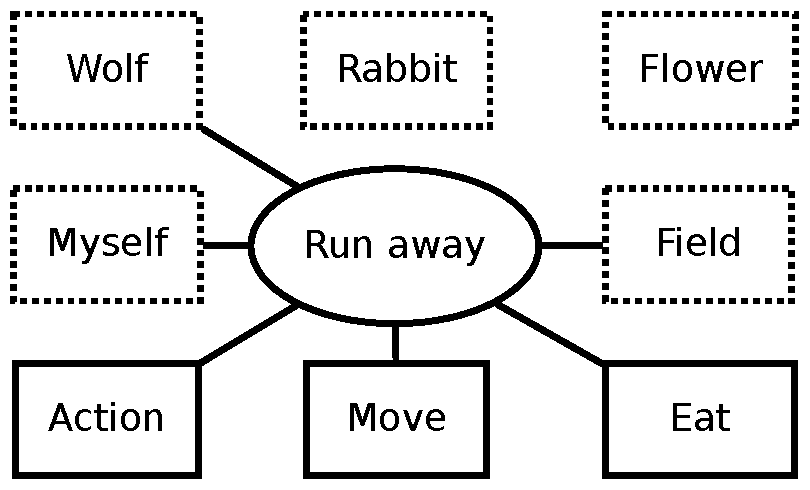
\includegraphics[keepaspectratio=true, scale=0.4]{run_away.pdf}
		\caption
		{
			\label{run_away_figure}
			A meta-knowledge module (circle one) about \textit{run away} behaviour linked to modules it combines.
		}
	\end{figure}
	
	\begin{example}
		\label{feed_example}
		A meta-knowledge module which describe the attack behaviour of wolf:\newline
		\newline
		\textbf{use\_module}("Myself").\newline
		\textbf{use\_module}("Rabbit").\newline
		\textbf{use\_module}("Flower").\newline
		\textbf{use\_module}("Field").\newline
		\textbf{use\_module}("Move").\newline
		\textbf{use\_module}("Eat").\newline
		\textbf{use\_module}("Action").
	\end{example}
	
	\begin{figure}
		\centering
		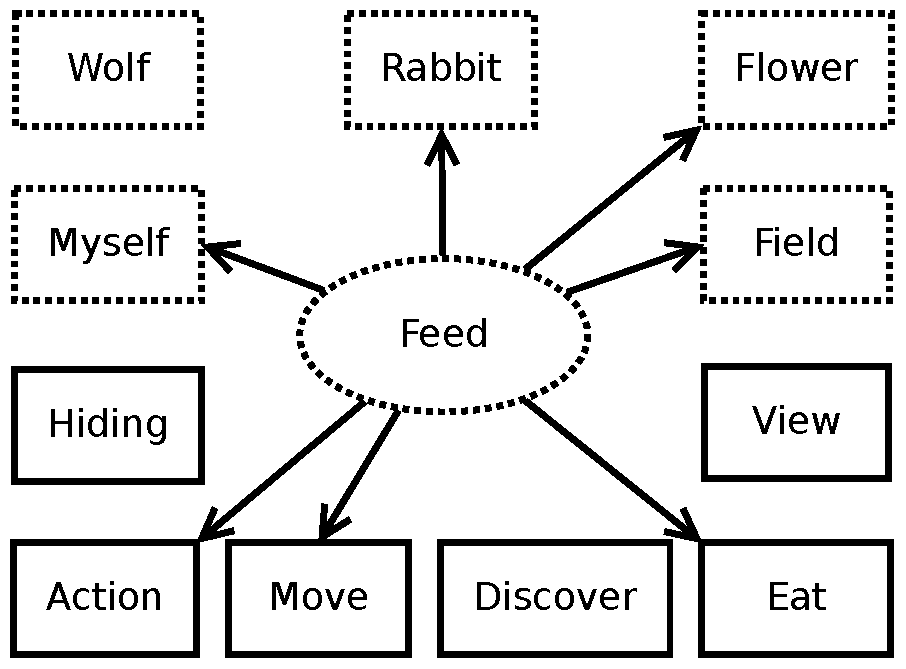
\includegraphics[keepaspectratio=true, scale=0.4]{feed.pdf}
		\caption
		{
			\label{feed_figure}
			A meta-knowledge module about \textit{feed} behaviour linked to modules it combines.
		}
	\end{figure}
	
	To represent more complex behaviour we can have meta-knowledge modules which have knowledge on other meta-knowledge modules.
	For example we can represent the survive behaviour of a rabbit with such module, like in example \ref{survive_example} and figure \ref{survive_figure}.
	If a rabbit spotted a wolf it will use the \emph{Run away} module otherwise it will use the \emph{Feed} module.
	Regarding the situation the survive behaviour will be run way or approach flower.
	Meta-knowledge modules allows to represent such dynamic behaviours which are dependent of the evolution of the environment.
	Figure \ref{behaviour_tree} represent rabbit behaviour by a meta-knowledge module tree.
	The behaviour of a rabbit is survive, regarding the situation a rabbit is hunted by a wolf or not.
	When hunted, a rabbit have to run away or try to hide by go out of view range of his predator.
	If there is no predator he will explore his environment to find flower and when one is spotted go to eat it.
	
	\begin{example}
		\label{survive_example}
		A meta-knowledge module which describe the hunting behaviour of wolf:\newline
		\newline
		predator $\leftarrow$ position(wolf,Position).\newline
		\textbf{use\_module}("Run away") $\leftarrow$ predator.\newline
		\textbf{use\_module}("Feed") $\leftarrow$ prey, not predator.\newline
	\end{example}
	
	\begin{figure}
		\centering
		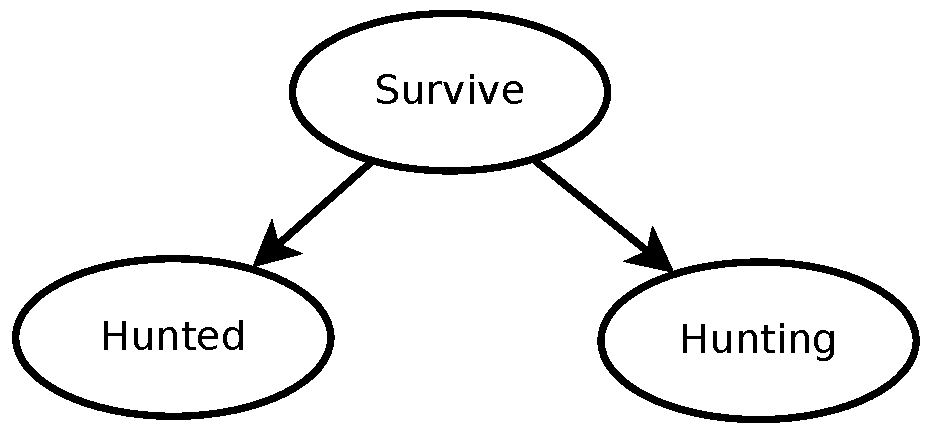
\includegraphics[keepaspectratio=true, scale=0.4]{survive.pdf}
		\caption
		{
			\label{survive_figure}
			A meta-knowledge module with knowledge about meta-knowledge module.
		}
	\end{figure}
	
	\begin{figure}
		\centering
		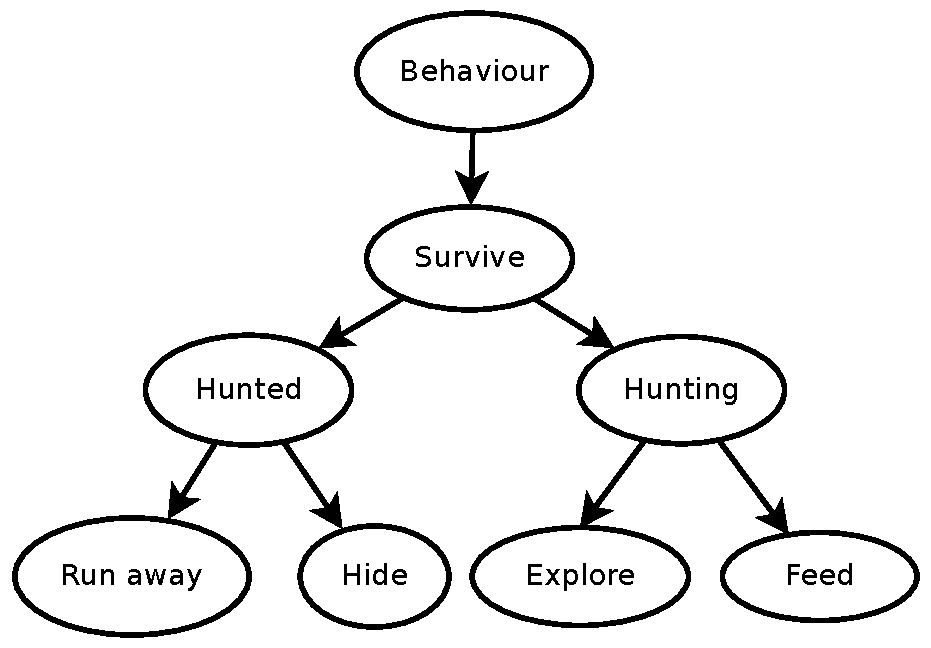
\includegraphics[keepaspectratio=true, scale=0.5]{behaviour_tree.pdf}
		\caption
		{
			\label{behaviour_tree}
			Representation of rabbit behaviour by a tree of meta-knowledge module.
		}
	\end{figure}
	
\subsection{Architecture}

	The previous section shows that ASP modules can represent background knowledge, observations and behaviours of an agent.
	To use this representation we define a reasoning architecture and a framework to use it in agent application.
	As show in figure \ref{framework_figure}, we divide agent reasoning into three phase : acquisition, deduction, action.
	
	Reasoning cycle start when agent sensors retrieve new observations, it's the beginning of the acquisition phase.
	This phase deals with new observations and their consequences on old ones.
	New observations are stored in corresponding observations modules and old ones are update.
	If a wolf see a rabbit at position P at time step T, he will store the information \textit{position(rabbit,P)} in module \textit{Rabbit}.
	Now at T+1 the wolf see position P but no rabbit are at P, then the wolf have to remove the fact \textit{position(rabbit,P)} from module \textit{Rabbit}.
	During acquisition phase, agent memory is update to make it consistent with new observations.
	
	After acquire observations, an agent will reason on what he can do regarding the current state of the world: it is the deduction phase.
	The purpose of this reasoning phase is to deduce what actions are possible to perform.
	Here we use an agent reasoning architecture based on ASP modules where meta-knowledge modules are use for meta-reasoning.
	Meta-knowledge modules use agent observations to define his behaviour step by step.
	Knowledge produce by module combination is keep in next reasoning steps, 
	it means that answer set of the last reasoning step contains all deduction of previous ones.
	These last answer set contains action and their consequences on the environment and the agent.
	
	The figure \ref{modular_knowledge} represent rabbit knowledge by an ASP modules graph where a node is an ASP module, 
	undirected edge represent the use of a module and directed edge represent reasoning decisions.
	Here meta-knowledge module \textit{Movement} is used to represent a module combination which produce movement actions of a rabbit,
	other ones represent his behaviour like in figure \ref{behaviour_tree}.
	The reasoning phase will start by using \textit{Behaviour} module which just specify to use \textit{Survive} one.
	By combining \textit{Survive} module and wolf observation the rabbit will decide if he is hunted or have to hunt.
	If he is hunted he will then combine \textit{Hunted} with wolf observations to decide if run away or hide is the best solution,
	for example if the wolf is very near it is very risky to hide then run away will be choose.
	If there is no wolf the rabbit will use \textit{Hunting} with flower observation, if there is no flower he will use \textit{Explore} module
	and \textit{View} to try to find something to eat (\textit{View} module should contains some knowledge about view range).
	If there is flower in his observations, a rabbit will use \textit{Feed} to produce actions will allows him to approach and eat flowers.
	
	Now the agent have to choose which actions to perform, it means choose an answer set which allows him to approach or reach his goals.
	To make this choice we can use constraint or use some modules to compute score to rank answer set.
	For example module \textit{Eat} can compute the number of action a predator have to perform to eat a prey.
	Then this module can be use by a rabbit to rank movement action to go far away from a wolf or to approach and eat a flower.
	After choosing the best answer set, corresponding actions are performed and 
	the cycle continue by the acquisition of the real effect of theses actions on the environment.

	\begin{figure}
		\centering
		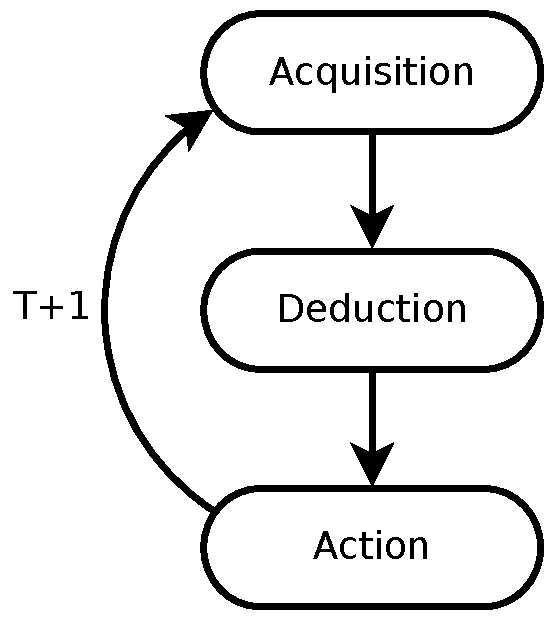
\includegraphics[keepaspectratio=true, scale=0.4]{framework.pdf}
		\caption
		{
			\label{framework_figure}
			Agent reasoning cycle.
		}
	\end{figure}

	\begin{figure}
		\centering
		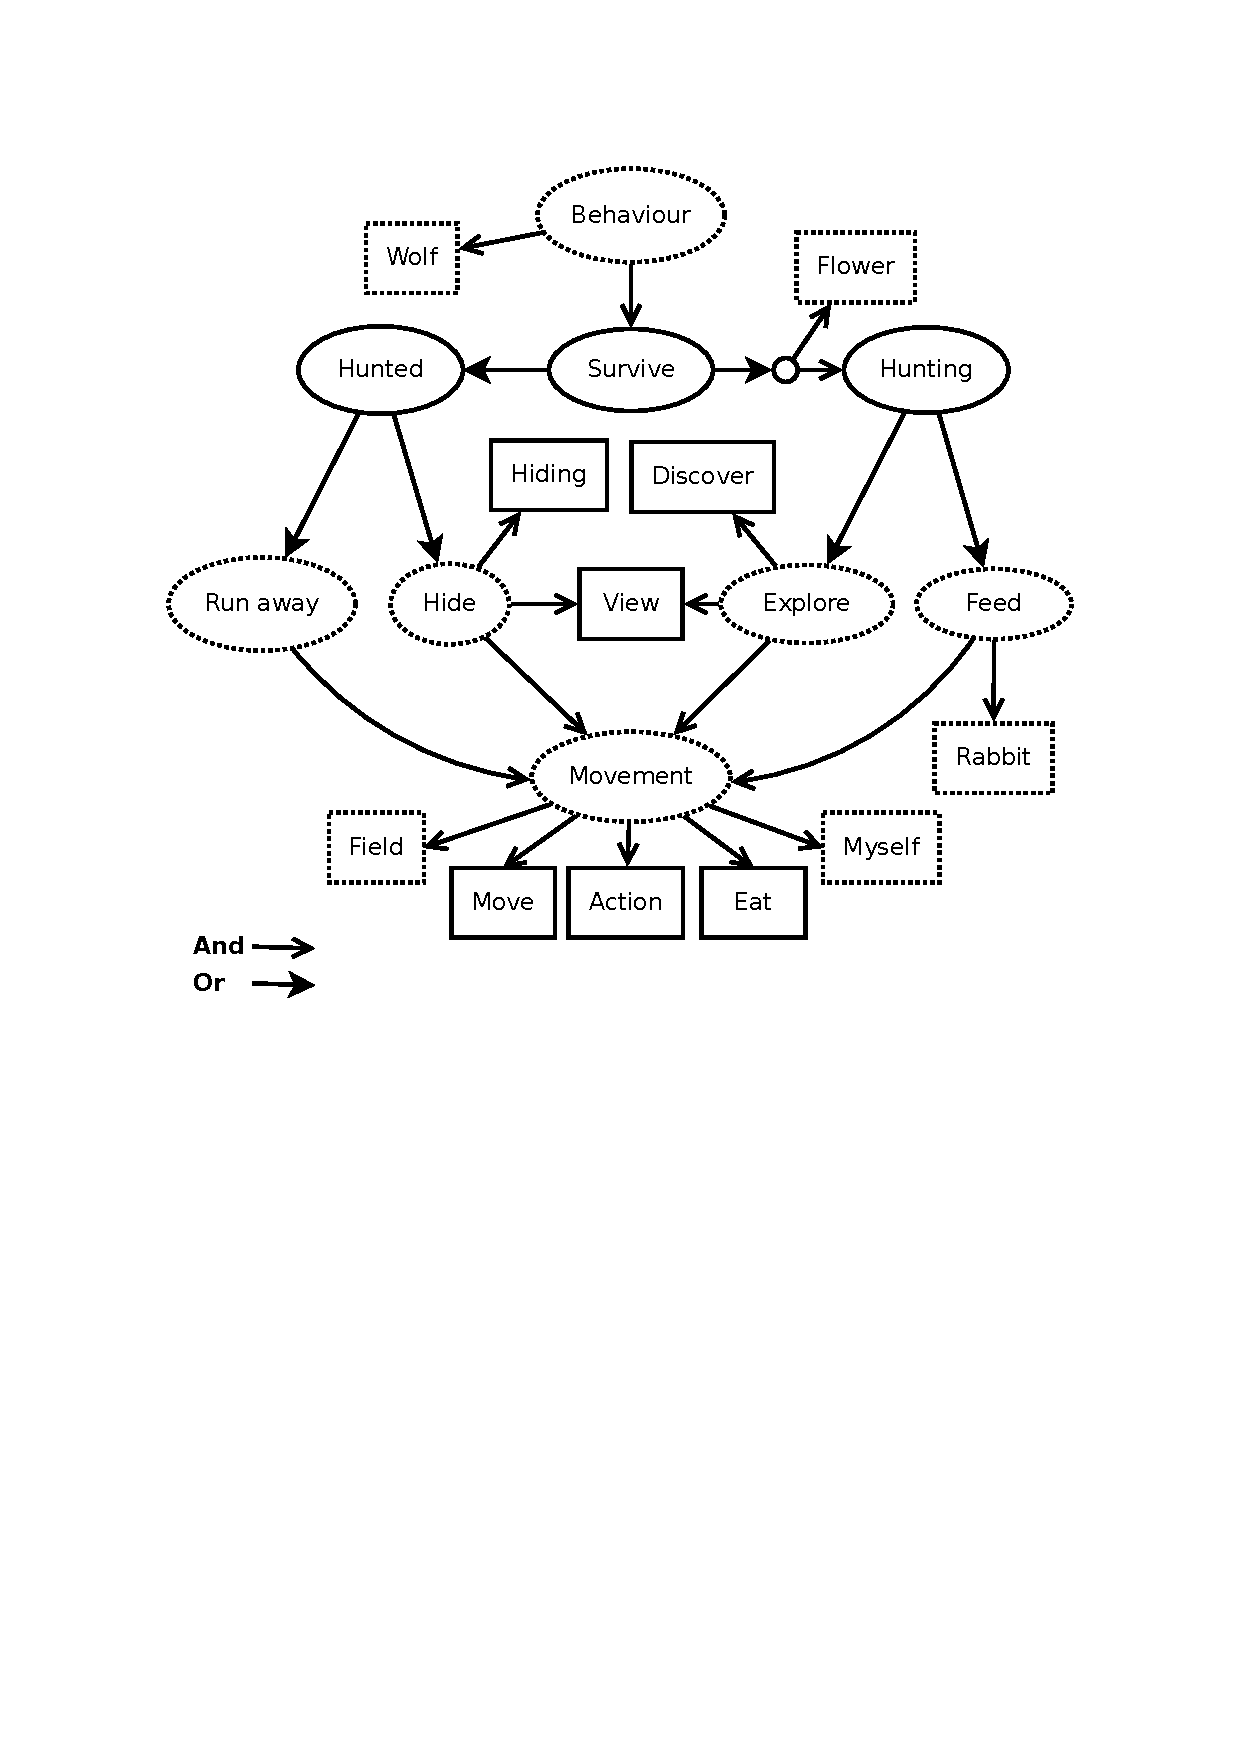
\includegraphics[keepaspectratio=true, scale=0.5]{modular_knowledge.pdf}
		\caption
		{
			\label{modular_knowledge}
			Representation of rabbit knowledge by an ASP modules graph.
		}
	\end{figure}
	
\section{Implementation}

	To allow an agent to use our method for reasoning in dynamic environment we implemented this framework.
	Algorithm \ref{framework_algorithm} represent a simplified version of this tool.
	
	Input is a set of modules and output is a set of answer set which contains actions that an agent can perform on its environment.
	It start by computing the combination of input modules and retrieve its answer sets by using the solver \emph{clingo}.
	Answer set are exploit in a deep first exploration by extracting keyword which define the combination of modules to use in the next reasoning step.
	When the answer set is totally parsed, we convert the current answer set into an ASP module and add it to the next combination of modules.
	Then, this combination is use for the next reasoning step and cycle continue.
	Finally, when there is no more module to combine it return a set of answer set.

	Let's take again the example of the figure \ref{modular_knowledge} and let's suppose that the rabbit just receive a set of new observation from its sensors.
	First our agent will combine theses new observations with the module \emph{Behaviour} to decide if he is hunted or have to hunt.
	Let's suppose that observations contains a wolf position, then the next combination of module to use is \{\emph{Hunted}\}.
	The wolf is too near to try to hide, so the next combination of module to use is \{\emph{Run away}\} which just specify to use \{\emph{Movement}\}.
	Finally this module will specify that the last combination of module to use is \{\emph{Myself}, \emph{Field}, \emph{Action}, \emph{Move}, \emph{Eat}\}.
	Then the algorithm will return all answer set of this combination, each answer will contain an movement action and its consequences, 
	for example the number of movement the wolf have to perform to catch the rabbit.
	
	In this example we can see that only a part of the knowledge is use for reasoning: 
	meta-knowledge modules \emph{Hide}, \emph{Hunting}, \emph{Explore} and \emph{Feed} are not used.
	Observations about flowers and knowledge about view are not used.
	The same knowledge can be represented in only one ASP program, but in this case all knowledge is use.
	Regarding this monolithic representation our method allows to reduce reasoning search space.
	
	Reasoning always finish when an agent use a module graph which is acyclic like in figure \ref{modular_knowledge}.
	To represent behaviours it is quite intuitive to make a tree of meta-knowledge modules, 
	where the root is the most abstract behaviour and deeper one are more specific.

	\begin{algorithm}
	\caption{Combine}
	\label{framework_algorithm}
	\begin{algorithmic}[1]
	\STATE INPUT : <M> M a set of ASP modules
	\STATE OUTPUT : AS a set of answer set
	\newline
	\STATE AS a set of answer set
	\newline
	\STATE AS $\leftarrow$ \textit{clingo}(M)
	\newline
	\FOR {each answer set S of AS}
		\STATE M $\leftarrow \emptyset$ 
		\newline
		\STATE // Extract keywords
		\FOR {every literal L of S}
			\IF {L = "use\_module(Module)"}
				\STATE M $\leftarrow$ M $\cup$ Module
				\STATE S $\leftarrow$ S $/$ L
			\ENDIF
		\ENDFOR
		\newline
		\IF {M $\neq$ $\emptyset$}
			\STATE // Add S to M as a module
			\STATE M $\leftarrow$ M $\cup$ module(S)
			\STATE combine(M)
		\ENDIF
	\ENDFOR
	\newline
	\RETURN AS
	\end{algorithmic}
	\end{algorithm}

\section{Experiments}

	To evaluate our work we implemented the algorithm \ref{framework_algorithm} and use it in a toy application based on the survival game example.
	In this application, the environment is a grid where agent are located on a square.
	Agents act turn by turn and have limited number of actions per turn.
	Theses actions can be: move to square or eat an agent.
	To eat his prey, a predator have to be on the same square.
	These experimental results focus on the reasoning time of a rabbit regarding a specific scenario.
	Here we compare modular and monolithic reasoning time: the first one needs multiple step to reach the module combination
	which correspond to the situation and the second one use directly the entire knowledge base.
	The figure \ref{modular_knowledge_experiment} represent the modular knowledge of the rabbit in these experiments.
	It is a simplified version where rabbit have two behaviours: \textit{run away} and \textit{feed}.
	Every scenarios concern a rabbit which has spotted a wolf and which reason about how to run away.
	The specificity of \textit{run away} behaviour is that it ignore observations about flowers. 
	
	Reasoning about flower is useless in these scenarios and can take a lot of time regarding the number of flower to consider.
	Here, flowers are used to illustrate unnecessary informations and how modular reasoning can avoid this kind of knowledge.
	
	The figure \ref{scenario_1} represent the first scenario, here there is no flower.
	In this scenario the rabbit just consider the movement he can perform regarding the distance between him and his predator.
	This scenario is used to evaluate the time we loose when modularity reasoning is not useful.
	
	The figure \ref{scenario_2}represent the second scenario, here there is 4 flowers.
	Here, monolithic reasoning consider movement regarding the wolf and these flowers.
	For each movement it compute the number of action the rabbit will need to eat each flowers.
	Modular reasoning perform the same reasoning as in the first scenario because it ignore flowers observations.
	
	The figure \ref{scenario_3} represent the third scenario, here our agent are in a field 25 flowers.
	Like in the second scenario, the monolithic reasoning lose time to reason about these flowers but the modular one does not.
	
	\begin{figure}
		\centering
		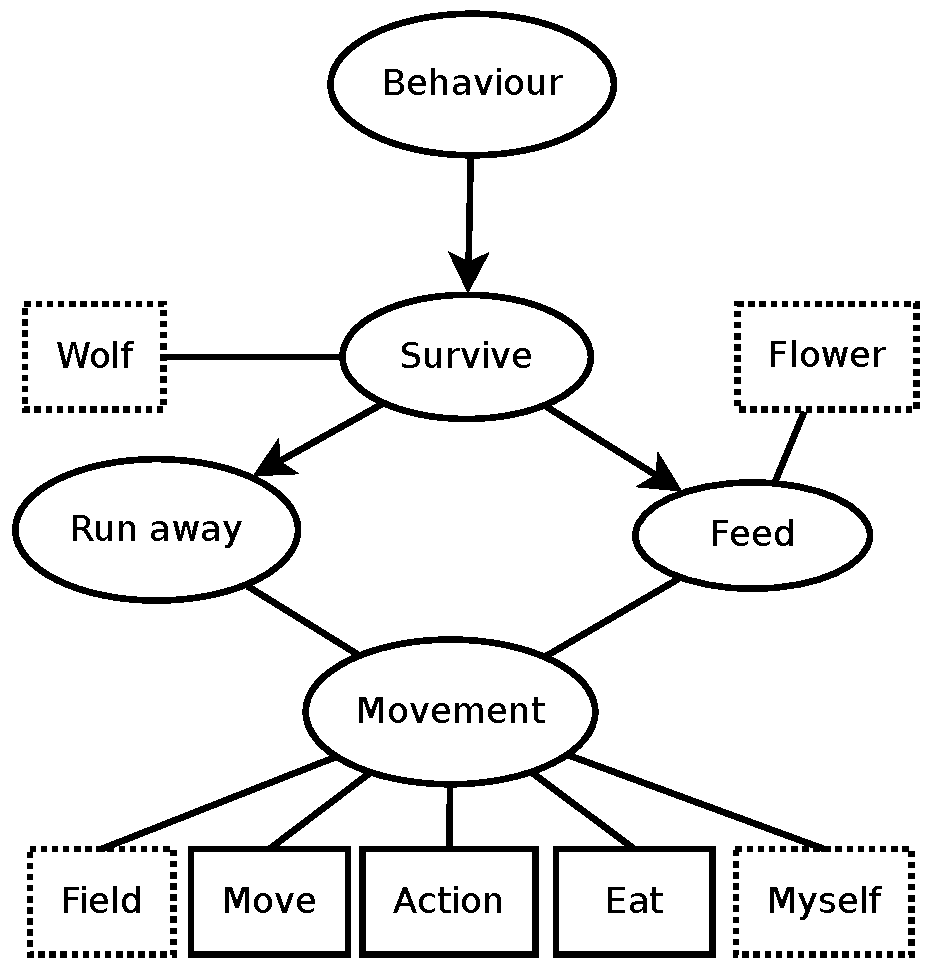
\includegraphics[keepaspectratio=true, scale=0.4]{modular_knowledge_experiment.pdf}
		\caption
		{
			\label{modular_knowledge_experiment}
			Representation of rabbit knowledge by an ASP modules graph.
		}
	\end{figure}
	
	\begin{figure}
		\centering
		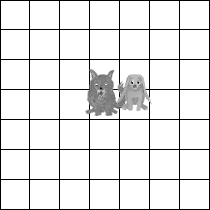
\includegraphics[keepaspectratio=true, scale=0.5]{scenario_1.png}
		\caption
		{
			\label{scenario_1}
			Scenario 1, a rabbit and a wolf.
		}
	\end{figure}

	\begin{figure}
		\centering
		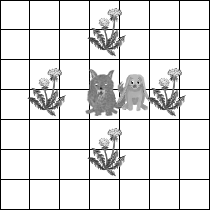
\includegraphics[keepaspectratio=true, scale=0.5]{scenario_2.png}
		\caption
		{
			\label{scenario_2}
			Scenario 2, a rabbit, a wolf and 4 flowers.
		}
	\end{figure}
	
	\begin{figure}
		\centering
		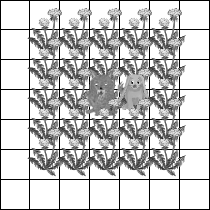
\includegraphics[keepaspectratio=true, scale=0.5]{scenario_3.png}
		\caption
		{
			\label{scenario_3}
			Scenario 3, a rabbit and a wolf in a field of 25 flowers.
		}
	\end{figure}

\section{Conclusions and Outlook}

	We provide a method based on ASP modules to design agent knowledge and reasoning.
	This representation allows to intuitively implements dynamic behaviours via meta-reasoning.
	We also provide a framework which allows agent reasoning by module combination.
	Regarding an equivalent monolithic representation, a first improvement of our method is the reduction of reasoning search space.
	Its also cause reduction of code size because modules are reusable for multiple purposes.
	
	In this paper, agent reasoning is very directed by meta-knowledge modules, 
	an interesting outlook will be to give the possibility to the agent to really choose which module combination he want to use.
	Make agent able to construct themselves a reasoning architecture like the one of figure \ref{modular_knowledge} is also an interesting research topic.
	Learning can also concern module content, an agent could choose to create new observations modules for storing specific information.
	Modular representation give new perspective for meta-reasoning and learning.
%
% The following two commands are all you need in the
% initial runs of your .tex file to
% produce the bibliography for the citations in your paper.
\bibliographystyle{abbrv}
\bibliography{ASP_Modules}  % sigproc.bib is the name of the Bibliography in this case
% You must have a proper ".bib" file
%  and remember to run:
% latex bibtex latex latex
% to resolve all references
%
% ACM needs 'a single self-contained file'!
%

\nocite{*}

\end{document}
